\documentclass{beamer}
\usepackage{fancyvrb}
\usepackage{color}
\usepackage{hyperref}
\hypersetup{
  colorlinks = false,
  urlcolor = blue,
  pdfauthor = {Alexander Mazurov},
  pdfkeywords = {scientific computing, system and distributing programming},
  pdftitle = {Optimization of software trigger and chib studies in LHCb}
  pdfsubject = {Optimization of software trigger and chib studies in LHCb},
  pdfpagemode = UseNone
}
% ============================================================================
\title{Update on $\chi_b$ studies}
\institute[University of Ferrara]{
  University of Ferrara, Italy\\
  \&\\
  CERN\\
  \texttt{alexander.mazurov@cern.ch}
}
% ============================================================================
\author[Sasha Mazurov]{Alexander (Sasha) Mazurov}
\date{19 December 2012}
\usetheme{Copenhagen}
\useoutertheme{infolines}
% ============================================================================
\begin{document}
\maketitle
\begin{frame}
% ----------------------------------------------------------------------------
\frametitle{My studies}
\begin{enumerate}
    \item Study of $\chi_{b}$ production.
    \item Measurement of $\chi_{b}(3P)$ mass.
\end{enumerate}
% ----------------------------------------------------------------------------
\end{frame}
% ============================================================================
\section{Study of $\chi_{b}$ production}
\subsection{Cross sections}
\begin{frame}
\frametitle{Cross sections formula}
In each $p_T(\Upsilon)$ bin calculate:
\begin{center}
$\frac{\sigma(\chi_{b} \rightarrow \Upsilon \gamma)}{\sigma(\Upsilon)} = \frac{N_{\chi_b \rightarrow \Upsilon \gamma}}{N_{\Upsilon}} \times \frac{\epsilon_{\Upsilon}}{\epsilon_{\chi_b \rightarrow \Upsilon \gamma}} = \frac{N_{\chi_b \rightarrow \Upsilon \gamma}}{N_{\Upsilon}} \times \frac{1}{\epsilon_{\gamma}^{reco}}$
\end{center}
\begin{itemize}
  \item Calculate for each $\Upsilon(nS), n=1,2,3$ and $\chi_b(mP), m=1,2,3$
  \item Get N from fits: $N_{\Upsilon}$ from  $m(\mu^+ \mu^-)$ and $N_{\chi_b \rightarrow \Upsilon \gamma}$ from [$m(\mu^+ \mu^- \gamma) - m(\mu^+ \mu^-)$] (for better resolution)
  \item Compute efficiency $\epsilon$  from Monte-Carlo simulation
  \item Luminosity = $1015 \pm 35 pb^{-1}$, data collected in year 2011.
\end{itemize}
\end{frame}

\begin{frame}[t]
\frametitle{Reconstruction}
Models were built on top of RooFit toolkit and unbinned maximum likelihood fits were performed.
\begin{columns}[t]
\column{.5\textwidth}
For $N_{\Upsilon}$:
invariant mass
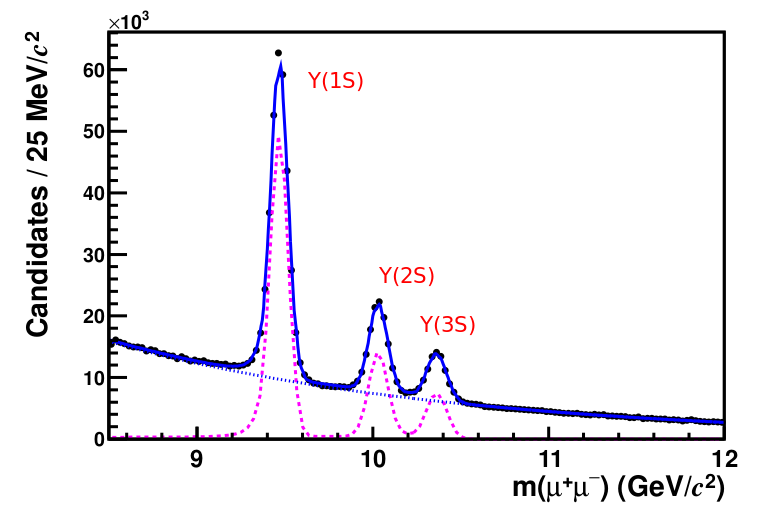
\includegraphics[height=.35\textheight]{images/ups.png}\\~\\
\begin{itemize}
  \item Signal: sum of 3 Crystal Ball functions
  \item Background: exponential function.
\end{itemize}
\column{.5\textwidth}
For $N_{\chi_{b} \rightarrow \Upsilon(1S) \gamma}$: mass difference
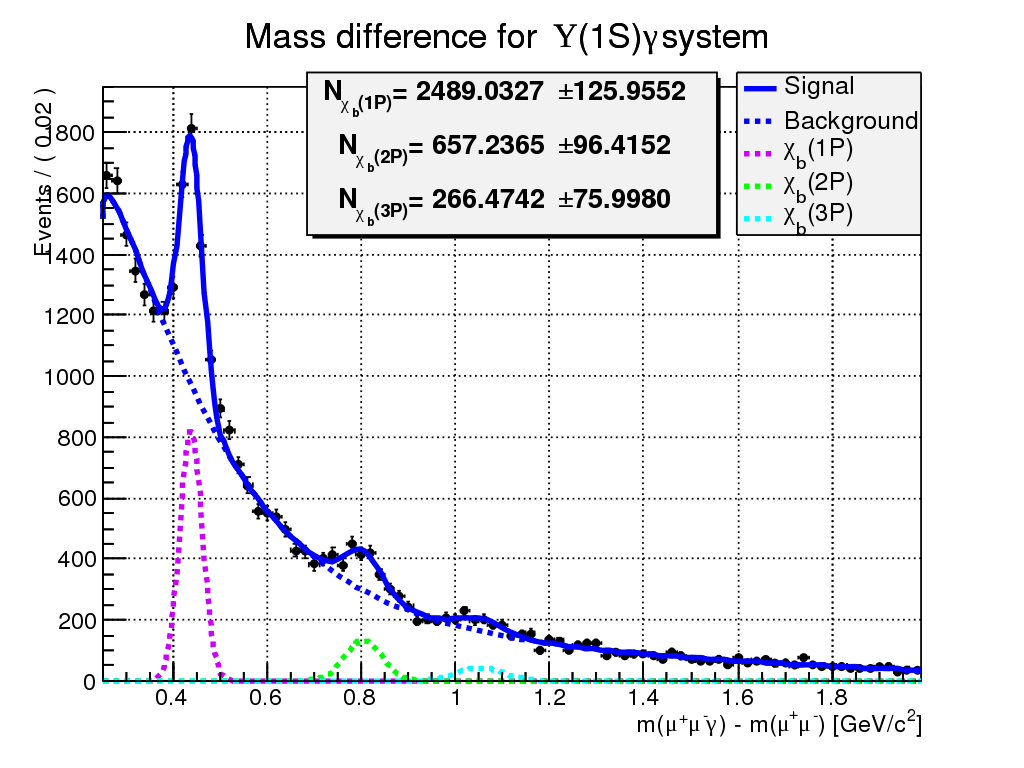
\includegraphics[height=.3\textheight]{images/fit.png}
\begin{itemize}
  \item Signal: 3 Gauss functions
  \item Background: $\sqrt{x} \times \left[e^{- \tau x} \times (c_1+a_1x+a_2x^2)\right] + \left[e^{-\tau x} \times (c_2+a_3x+a_4x^2)\right]$
\end{itemize}
(not enough resolution to separate $\chi_{b(0,1,2)}$)
\end{columns}
\end{frame}

\begin{frame}
\frametitle{Number of $\chi_b(NP) \rightarrow \Upsilon(1S)$ decays}
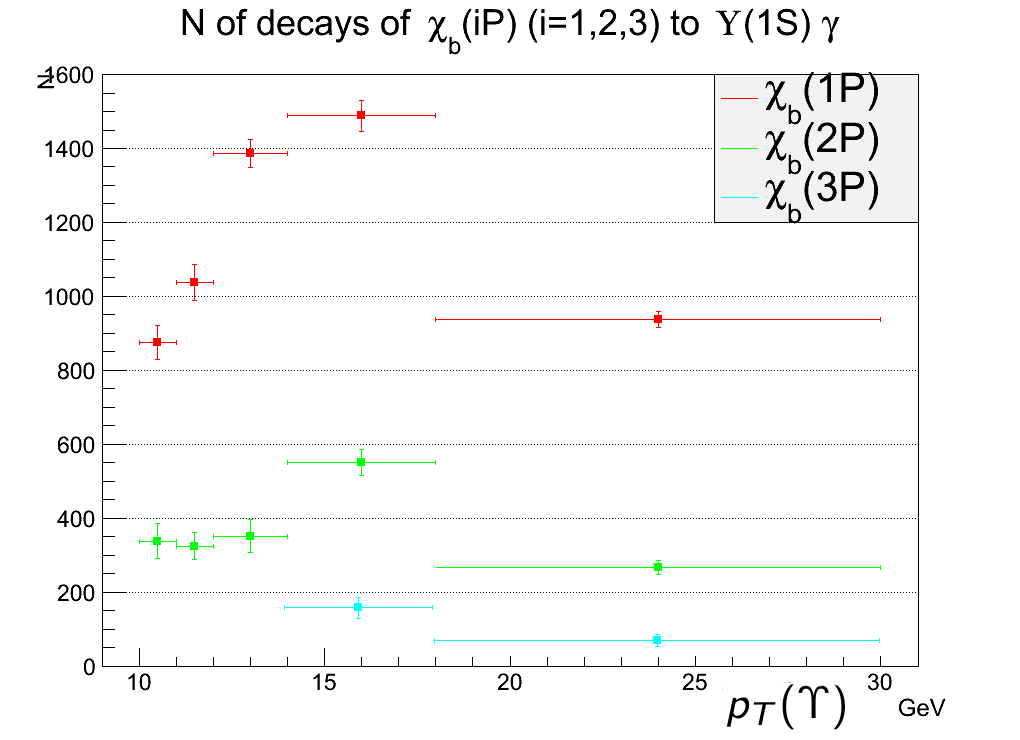
\includegraphics[width=.9\textwidth]{images/spectr.png}
\end{frame}
\begin{frame}

\frametitle{Monte-Carlo}
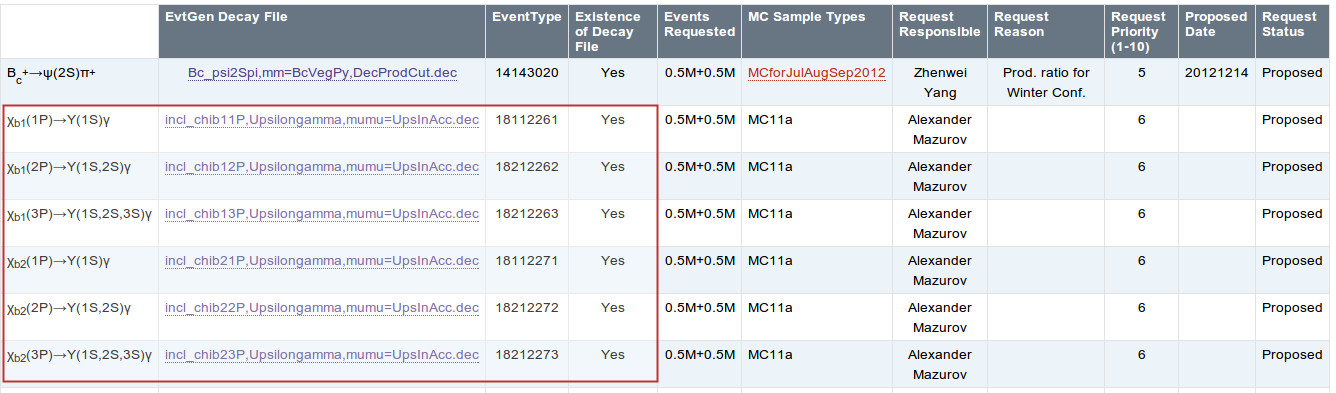
\includegraphics[width=.9\textwidth]{images/mcdkfiles.png}
\begin{itemize}
  \item Decay files were released (Gen/DecFiles v25r20).
  \item Will be produced during Xmass.
\end{itemize}
\end{frame}

\begin{frame}
\frametitle{$\chi_{b} \rightarrow \Upsilon(2S,3S)$}
\begin{columns}[T]
\column{.5\textwidth}
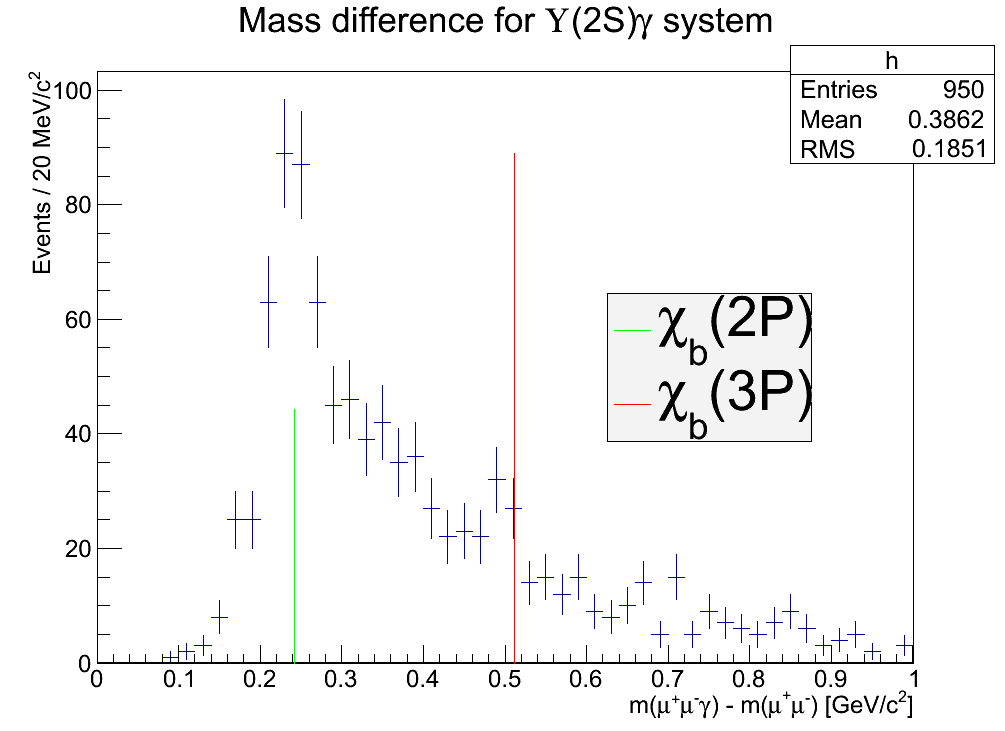
\includegraphics[width=.9\textwidth]{images/chibY2S.png}\\~\\
\column{.5\textwidth}
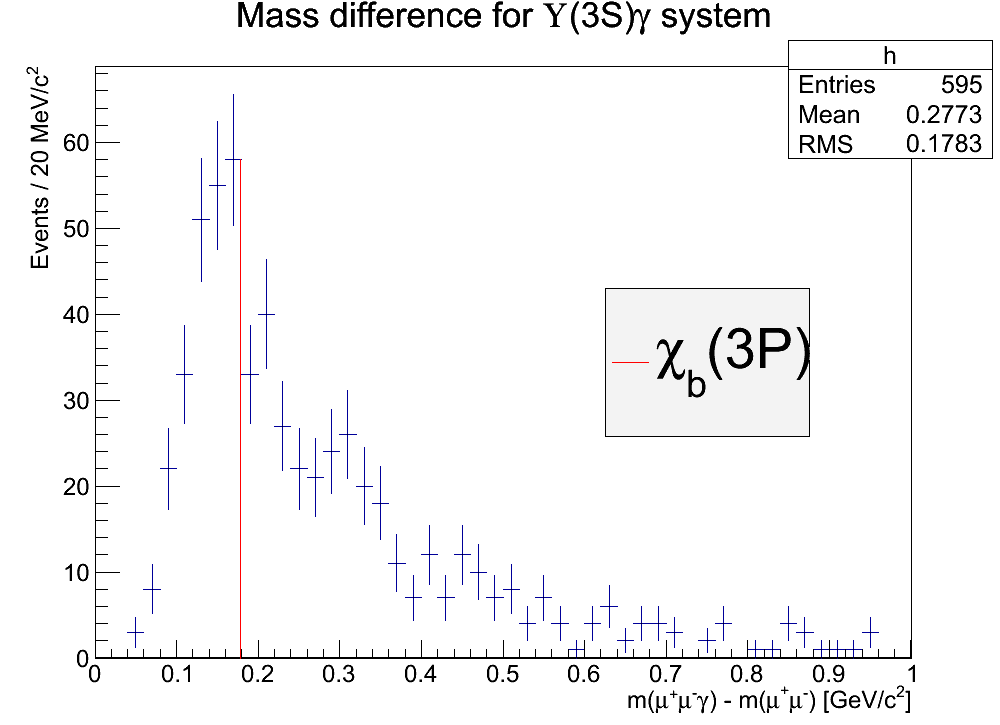
\includegraphics[width=.9\textwidth]{images/chibY3S.png}\\~\\
\end{columns}
\end{frame}

\subsection{Measurement of $\chi_{b}(3P)$ mass}
\begin{frame}
\begin{exampleblock}{}
    \begin{center}
        {\huge Measurement of $\chi_{b}(3P)$ mass}
    \end{center}
\end{exampleblock}
\end{frame}
\begin{frame}
\frametitle{Selection optimization}
Background subtraction
\begin{columns}[c]
\column{.5\textwidth}
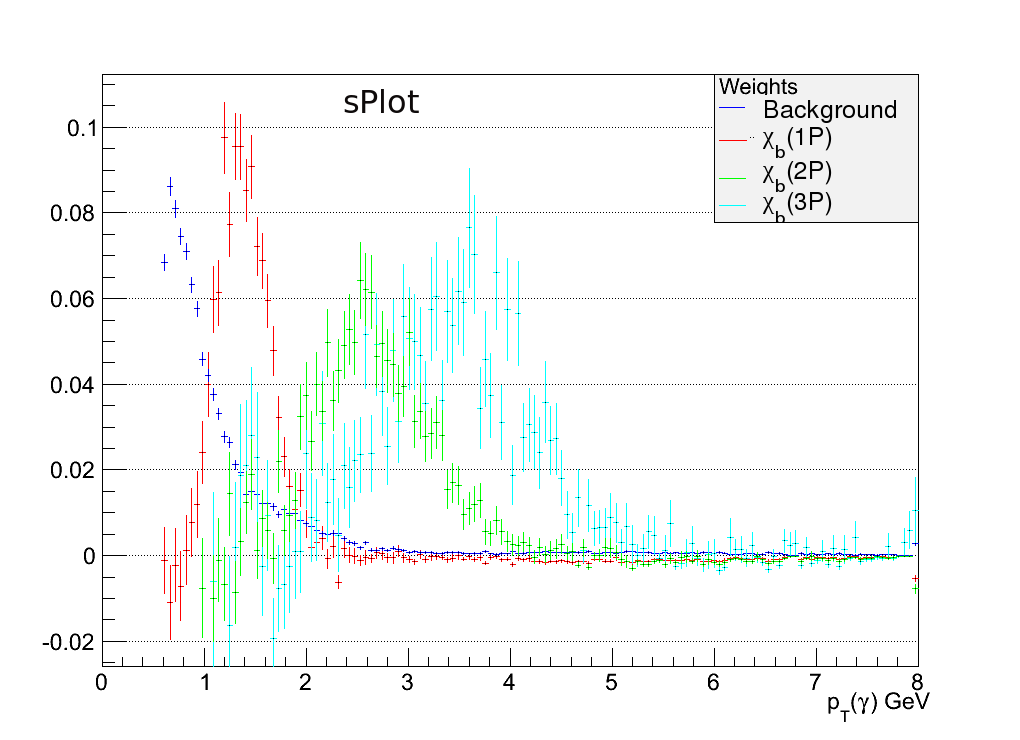
\includegraphics[width=\textwidth]{images/splot.png}
\column{.5\textwidth}
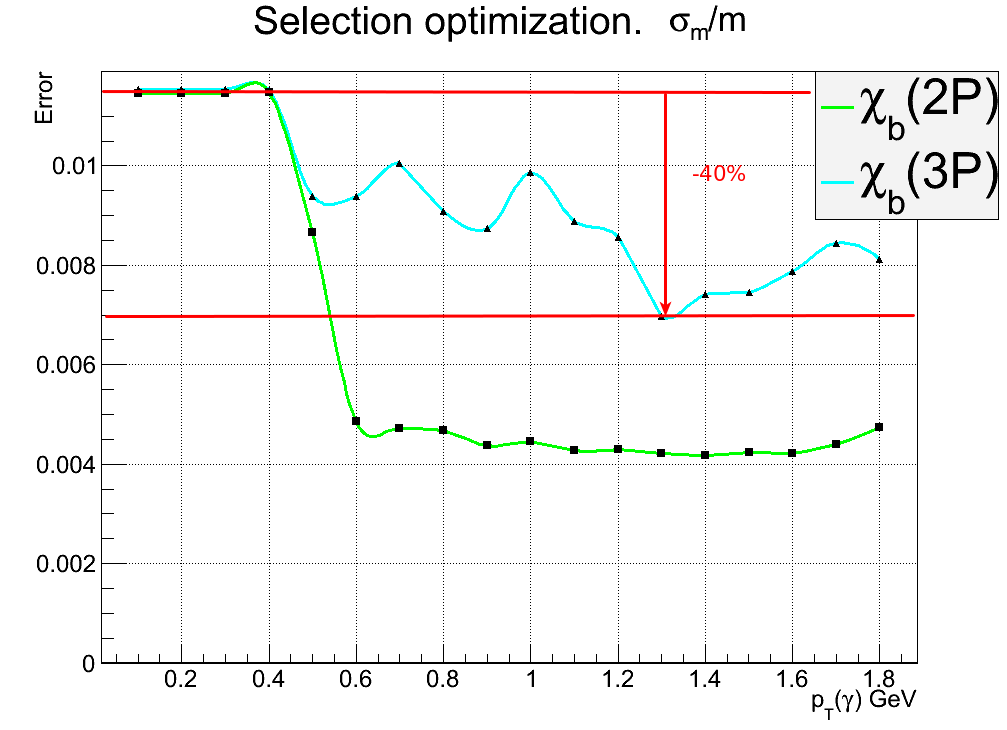
\includegraphics[width=\textwidth]{images/plot_rerr_m3p.png}
\end{columns}
\begin{itemize}
  \item We can reduce the background by tightening cut on $p_T(\gamma)$
  \item Can make a precise measurement of $m_{\chi_b(3P)}$
\end{itemize}
\end{frame}

\begin{frame}[t]
\frametitle{Very preliminary results}
\begin{columns}[T]
\column{.5\textwidth}
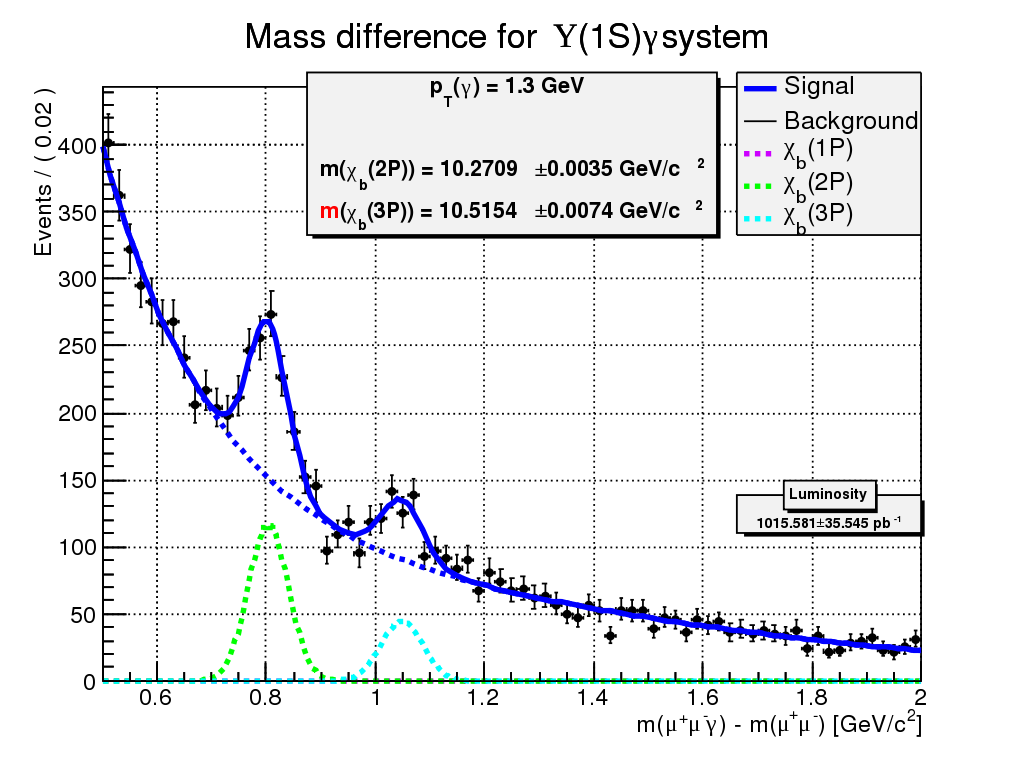
\includegraphics[height=.4\textheight]{images/m3p.png}\\~\\
\column{.5\textwidth}
Next steps:

\begin{itemize}
  \item Determine systematic errors
  \item Photon energy calibration
\end{itemize}
\end{columns}
\begin{tabular}{|l|c|c|}\hline
              &  $m_{\chi_b(2P)} [GeV/c^2]$ & $m_{\chi_b(3P)} [GeV/c^2]$\\ \hline
ATLAS         &                             & $10.530 \pm 0.0050$\\
D0            &                             & $10.551 \pm 0.0140$\\
LHCb (prev)   &  $10.2660 \pm 0.0060$       & $10.535 \pm 0.0100$\\ \hline
\textcolor{blue}{This study} & $~~~~10.2709 \pm 0.0035_{stat}$ & $~~~~10.515 \pm 0.0074_{stat}$ \\ \hline
% &  $10.2709 \pm 0.0035
\end{tabular}
\end{frame}

\begin{frame}
\frametitle{Summary}
\begin{enumerate}
\item Studying the production of $\chi_b$ particles in LHCb, through the reconstruction of $\chi_b \rightarrow \Upsilon \gamma$ decays, with the $\Upsilon$ decaying to $\mu^+ \mu^-$.
\item Determined $\chi_b \rightarrow \Upsilon(1S) \gamma$ yields as a function of $p_{T}(\Upsilon(1S))$.
\item Measured  mass of the $\chi_b(3P)$ state, which has been recently observed at LHC and TeVatron.
\item Finalize analysis (efficiencies, other decays,...).
\end{enumerate}
\end{frame}
\end{document}
